\section{Gestionnaire des utilisateurs}

Cette section décrit comment gérer les utilisateurs par un membre du staff. Pour accéder à cette page, l'utilisateur doit avoir la permission de gérer les utilisateurs (voir la section "Gestionnaire des permissions").\newline

Le gestionnaire des utilisateur permet de gérer les utilisateurs. En particulier, il est possible de modifier les informations d'un utilisateur.

\begin{figure}[H]
\centering
\includegraphics[scale=0.15]{user_images/staff/GererUtilisateurs/001.jpg}
\caption{Gestionnaire des utilisateurs}
\end{figure}

Cette page est divisée en deux parties: à droite, une liste des utilisateurs, à gauche, des critères de recherche pour affiner la liste des utilisateurs à droite. En bas à gauche, il est possible d'exporter la liste des utilisateurs au format CSV, ou bien uniquement la liste des adresses (toujours au format CSV).

\subsection{Consulter un utilisateur}

Pour consulter à un utilisateur, il faut cliquer sur l'entrée de la liste des utilisateurs à droite de l'écran correspondant à cet utilisateur.

\begin{figure}[H]
\centering
\includegraphics[scale=0.15]{user_images/staff/GererUtilisateurs/ConsulterUtilisateur/001.jpg}
\caption{Consulter un utilisateur, étape 1}
\end{figure}

On accède ensuite à la page de l'utilisateur, qui reprend les informations du joueurs, ainsi que les tournois inscrits et les terrains possédés.

\begin{figure}[H]
\centering
\includegraphics[scale=0.15]{user_images/staff/GererUtilisateurs/ConsulterUtilisateur/002.jpg}
\caption{Consulter un utilisateur, étape 2}
\end{figure}

\subsection{Editer un utilisateur}

Pour éditer un utilisateur, il faut accéder à la page de cet utilisateur, comme expliqué précédemment dans la sous-section "Consulter un utilisateur".

À partir de la page de l'utilisateur à éditer, cliquez sur le bouton "Modifier informations" pour accéder à la modification des informations de l'utilisateur.

\begin{figure}[H]
\centering
\includegraphics[scale=0.15]{user_images/staff/GererUtilisateurs/ModifierUtilisateur/001.jpg}
\caption{Editer un utilisateur, étape 1}
\end{figure}

Une boîte de dialogue, assez complexe, contient un formulaire pré-rempli des informations actuelles de l'utilisateur. Les champs indiqués par une étoile (*) sont obligatoires, et ne peuvent pas être vides.

\begin{figure}[H]
\centering
\includegraphics[scale=0.15]{user_images/staff/GererUtilisateurs/ModifierUtilisateur/002.jpg}
\caption{Editer un utilisateur, étape 2}
\end{figure}

Après avoir modifiés certains champs, comme ici le GSM, le numéro, et le classement, cliquez sur le bouton "Sauver" pour valider les modifications.

\begin{figure}[H]
\centering
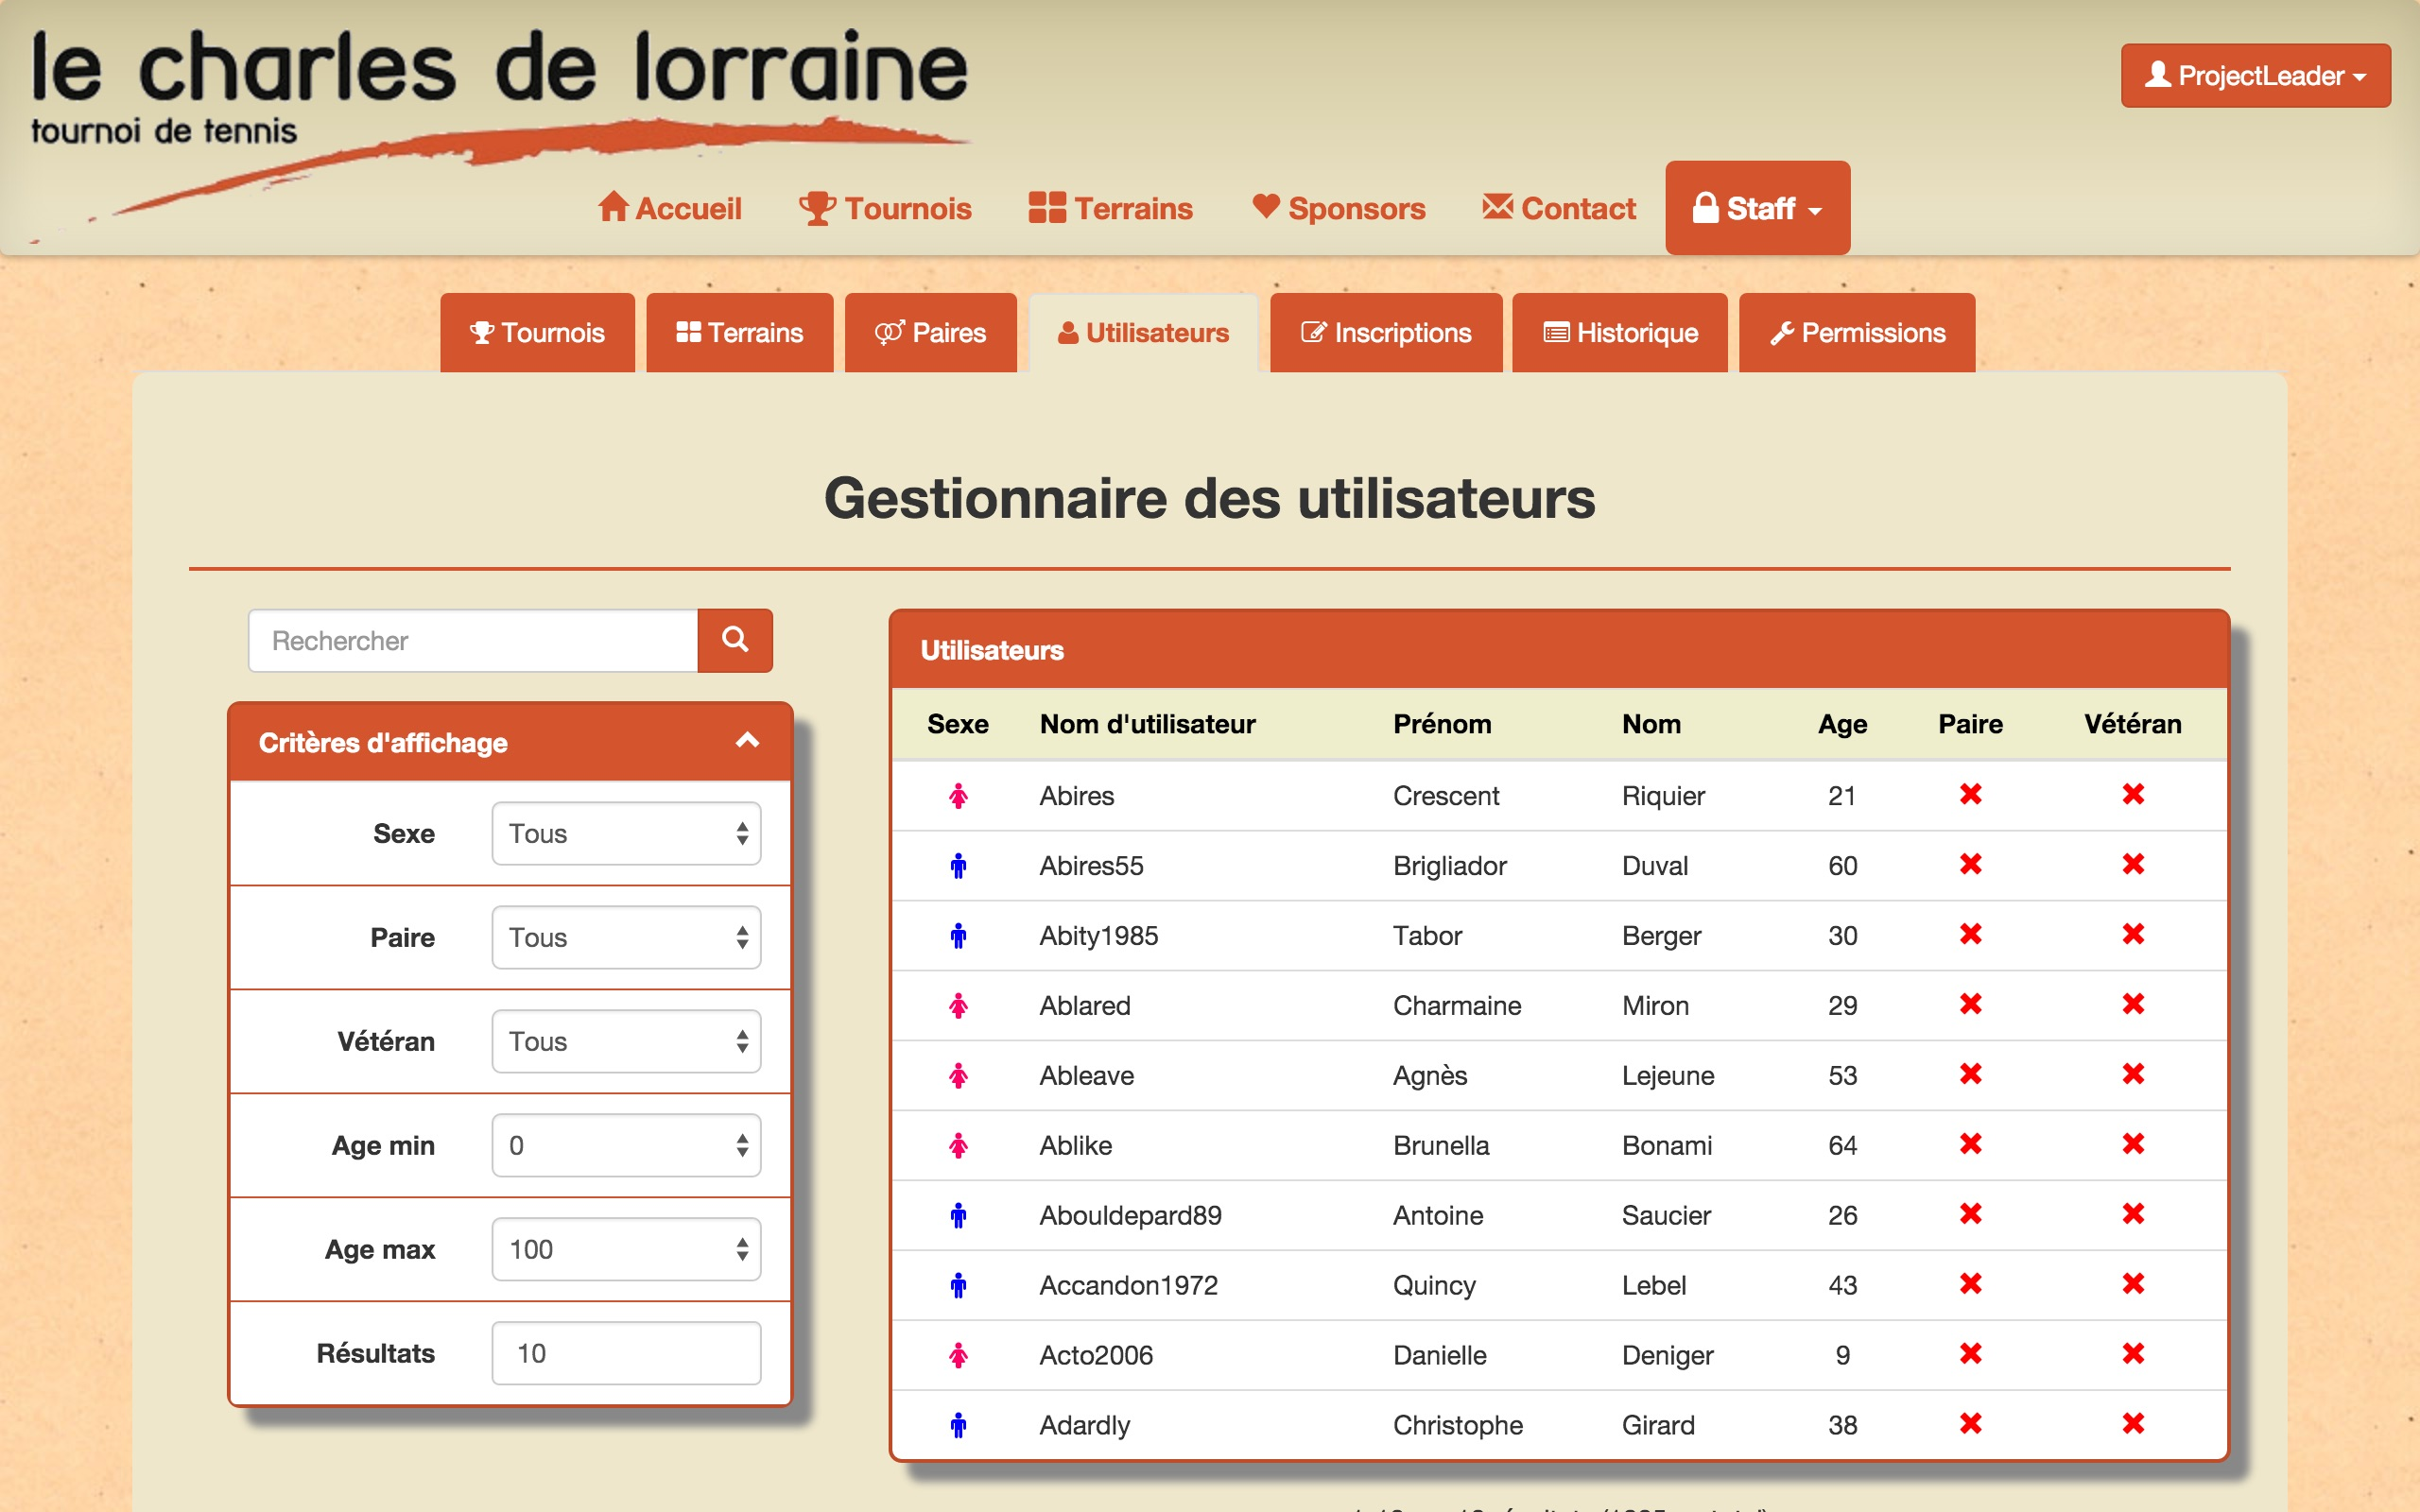
\includegraphics[scale=0.15]{user_images/staff/GererUtilisateurs/ModifierUtilisateur/003.jpg}
\caption{Editer un utilisateur, étape 3}
\end{figure}

Après avoir appliqué les modifications des informations de l'utilisateur, un message vert signale la bonne modification des informations de l'utilisateur.

\begin{figure}[H]
\centering
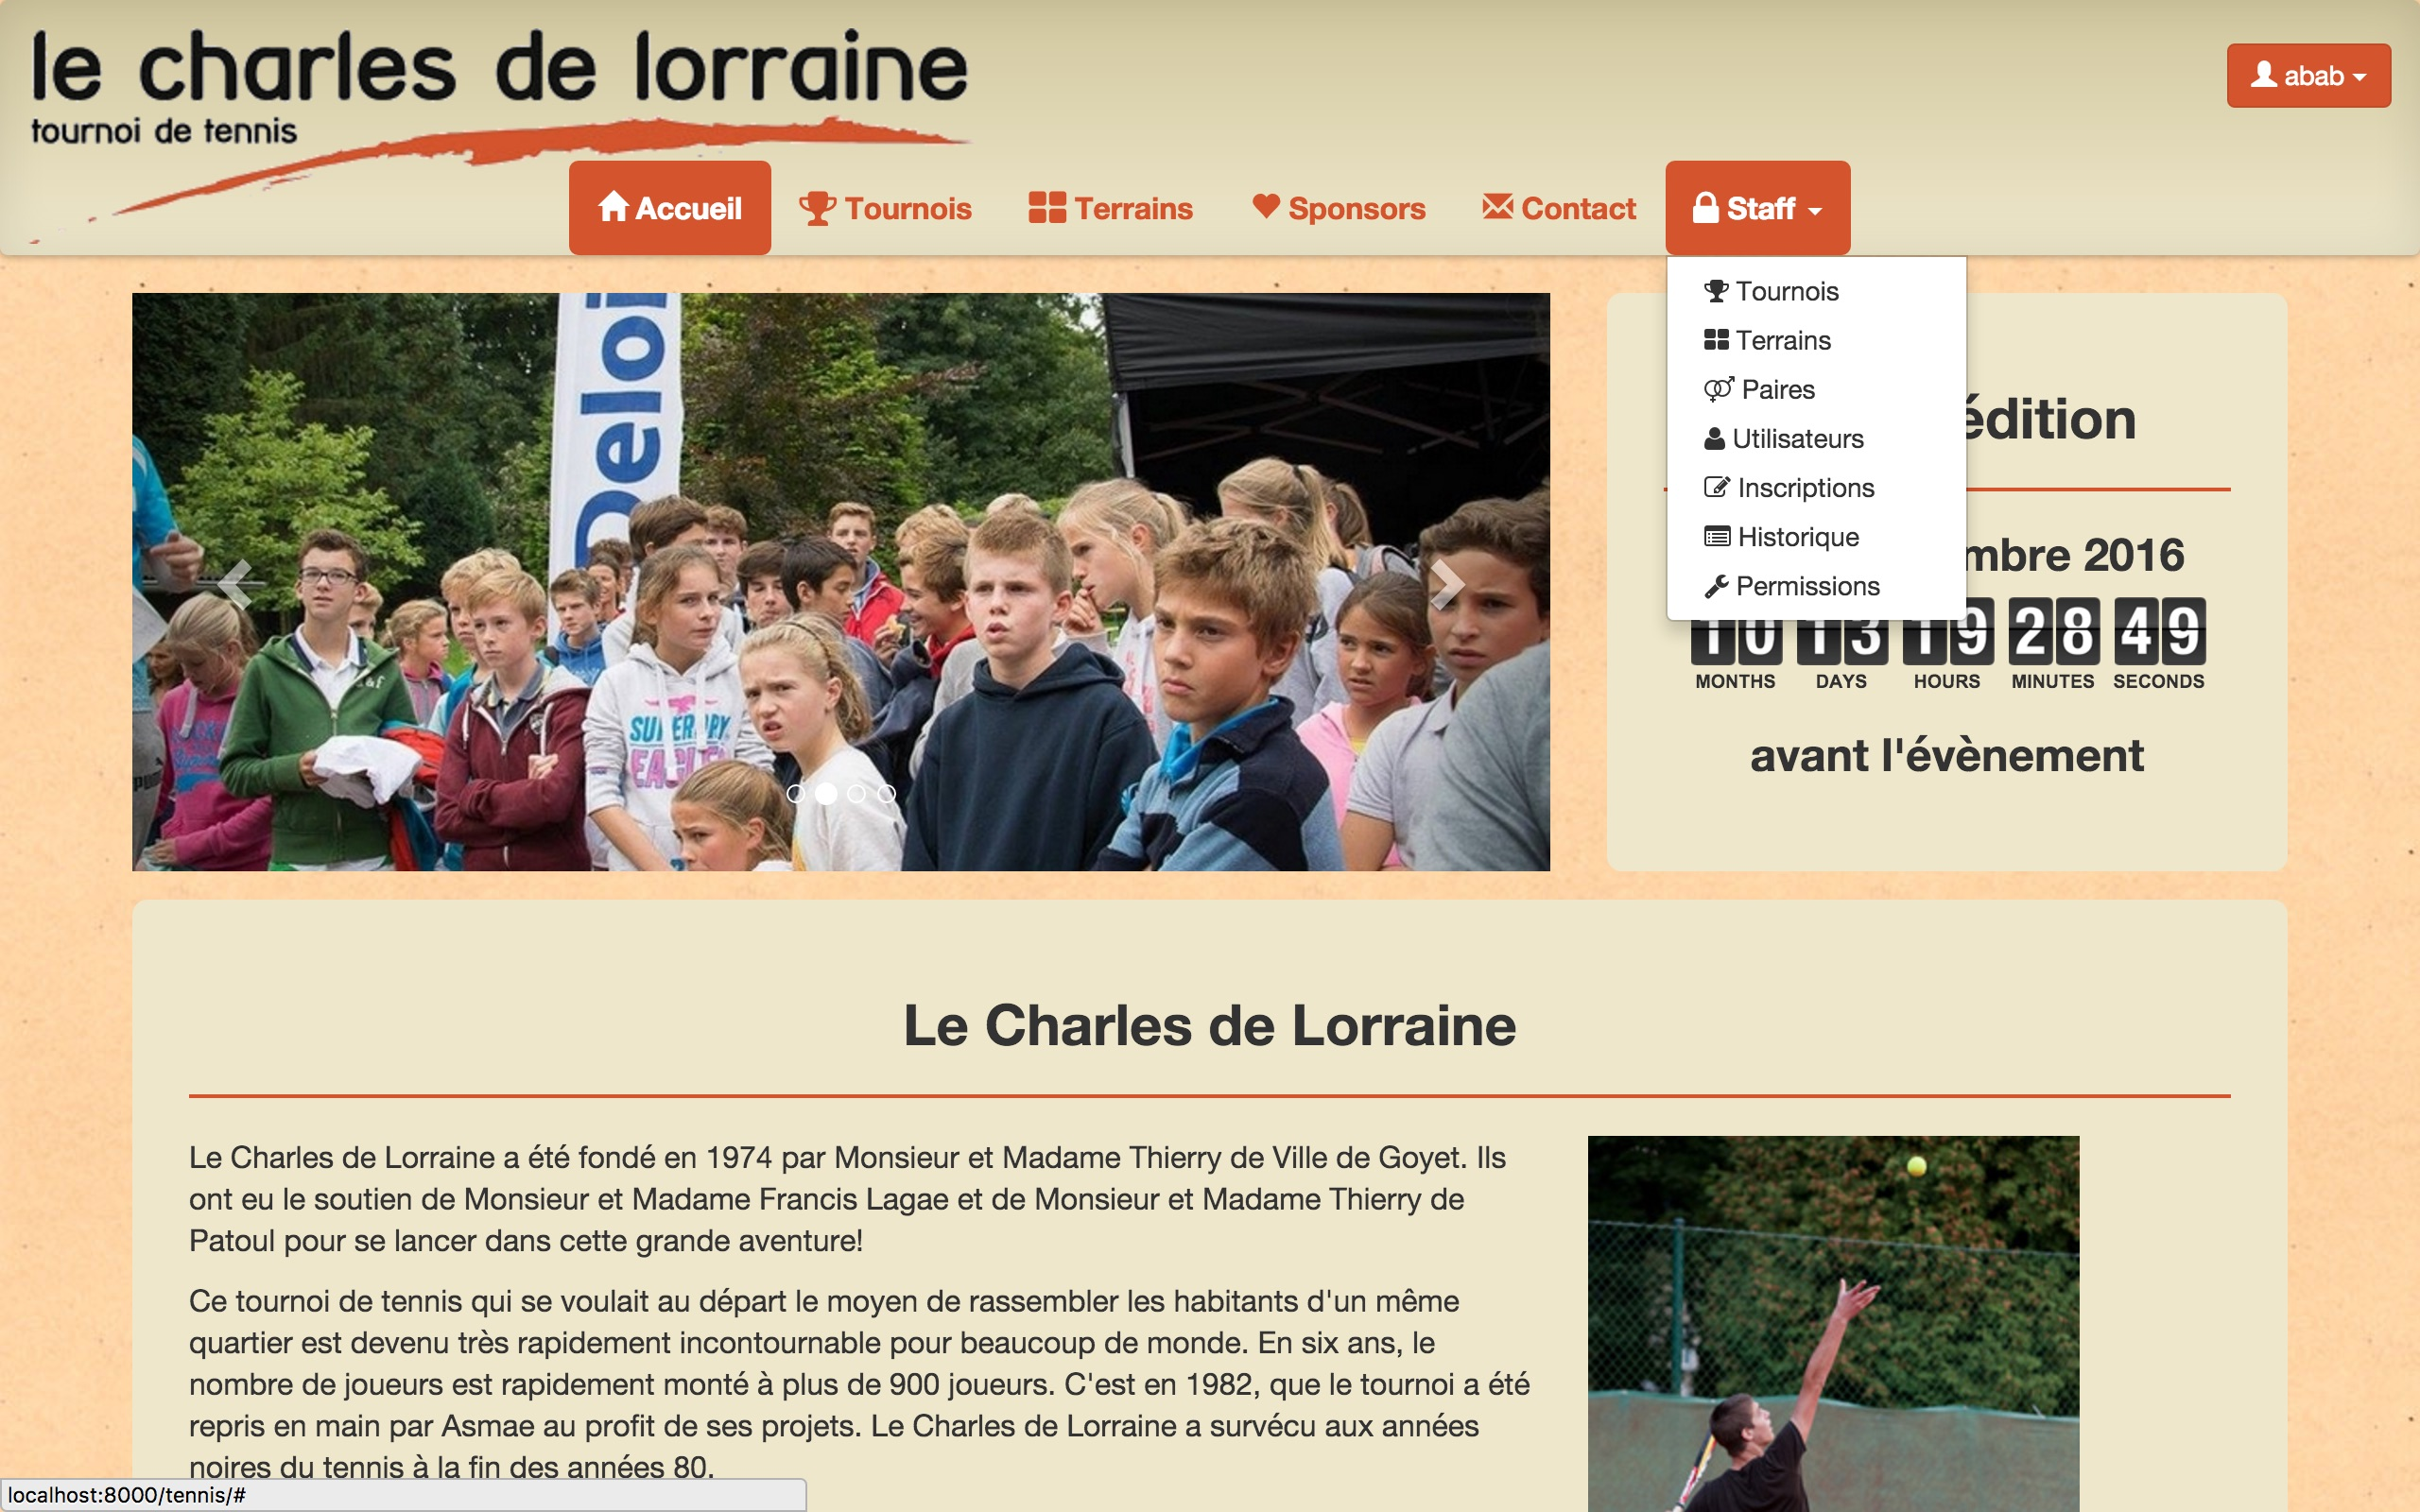
\includegraphics[scale=0.15]{user_images/staff/GererUtilisateurs/ModifierUtilisateur/004.jpg}
\caption{Editer un utilisateur, étape 4}
\end{figure}

En bas de la page de l'utilisateur, l'historique des modifications sur l'utilisateur confirme, à nouveau, que l'utilisateur a été récemment modifié.

\begin{figure}[H]
\centering
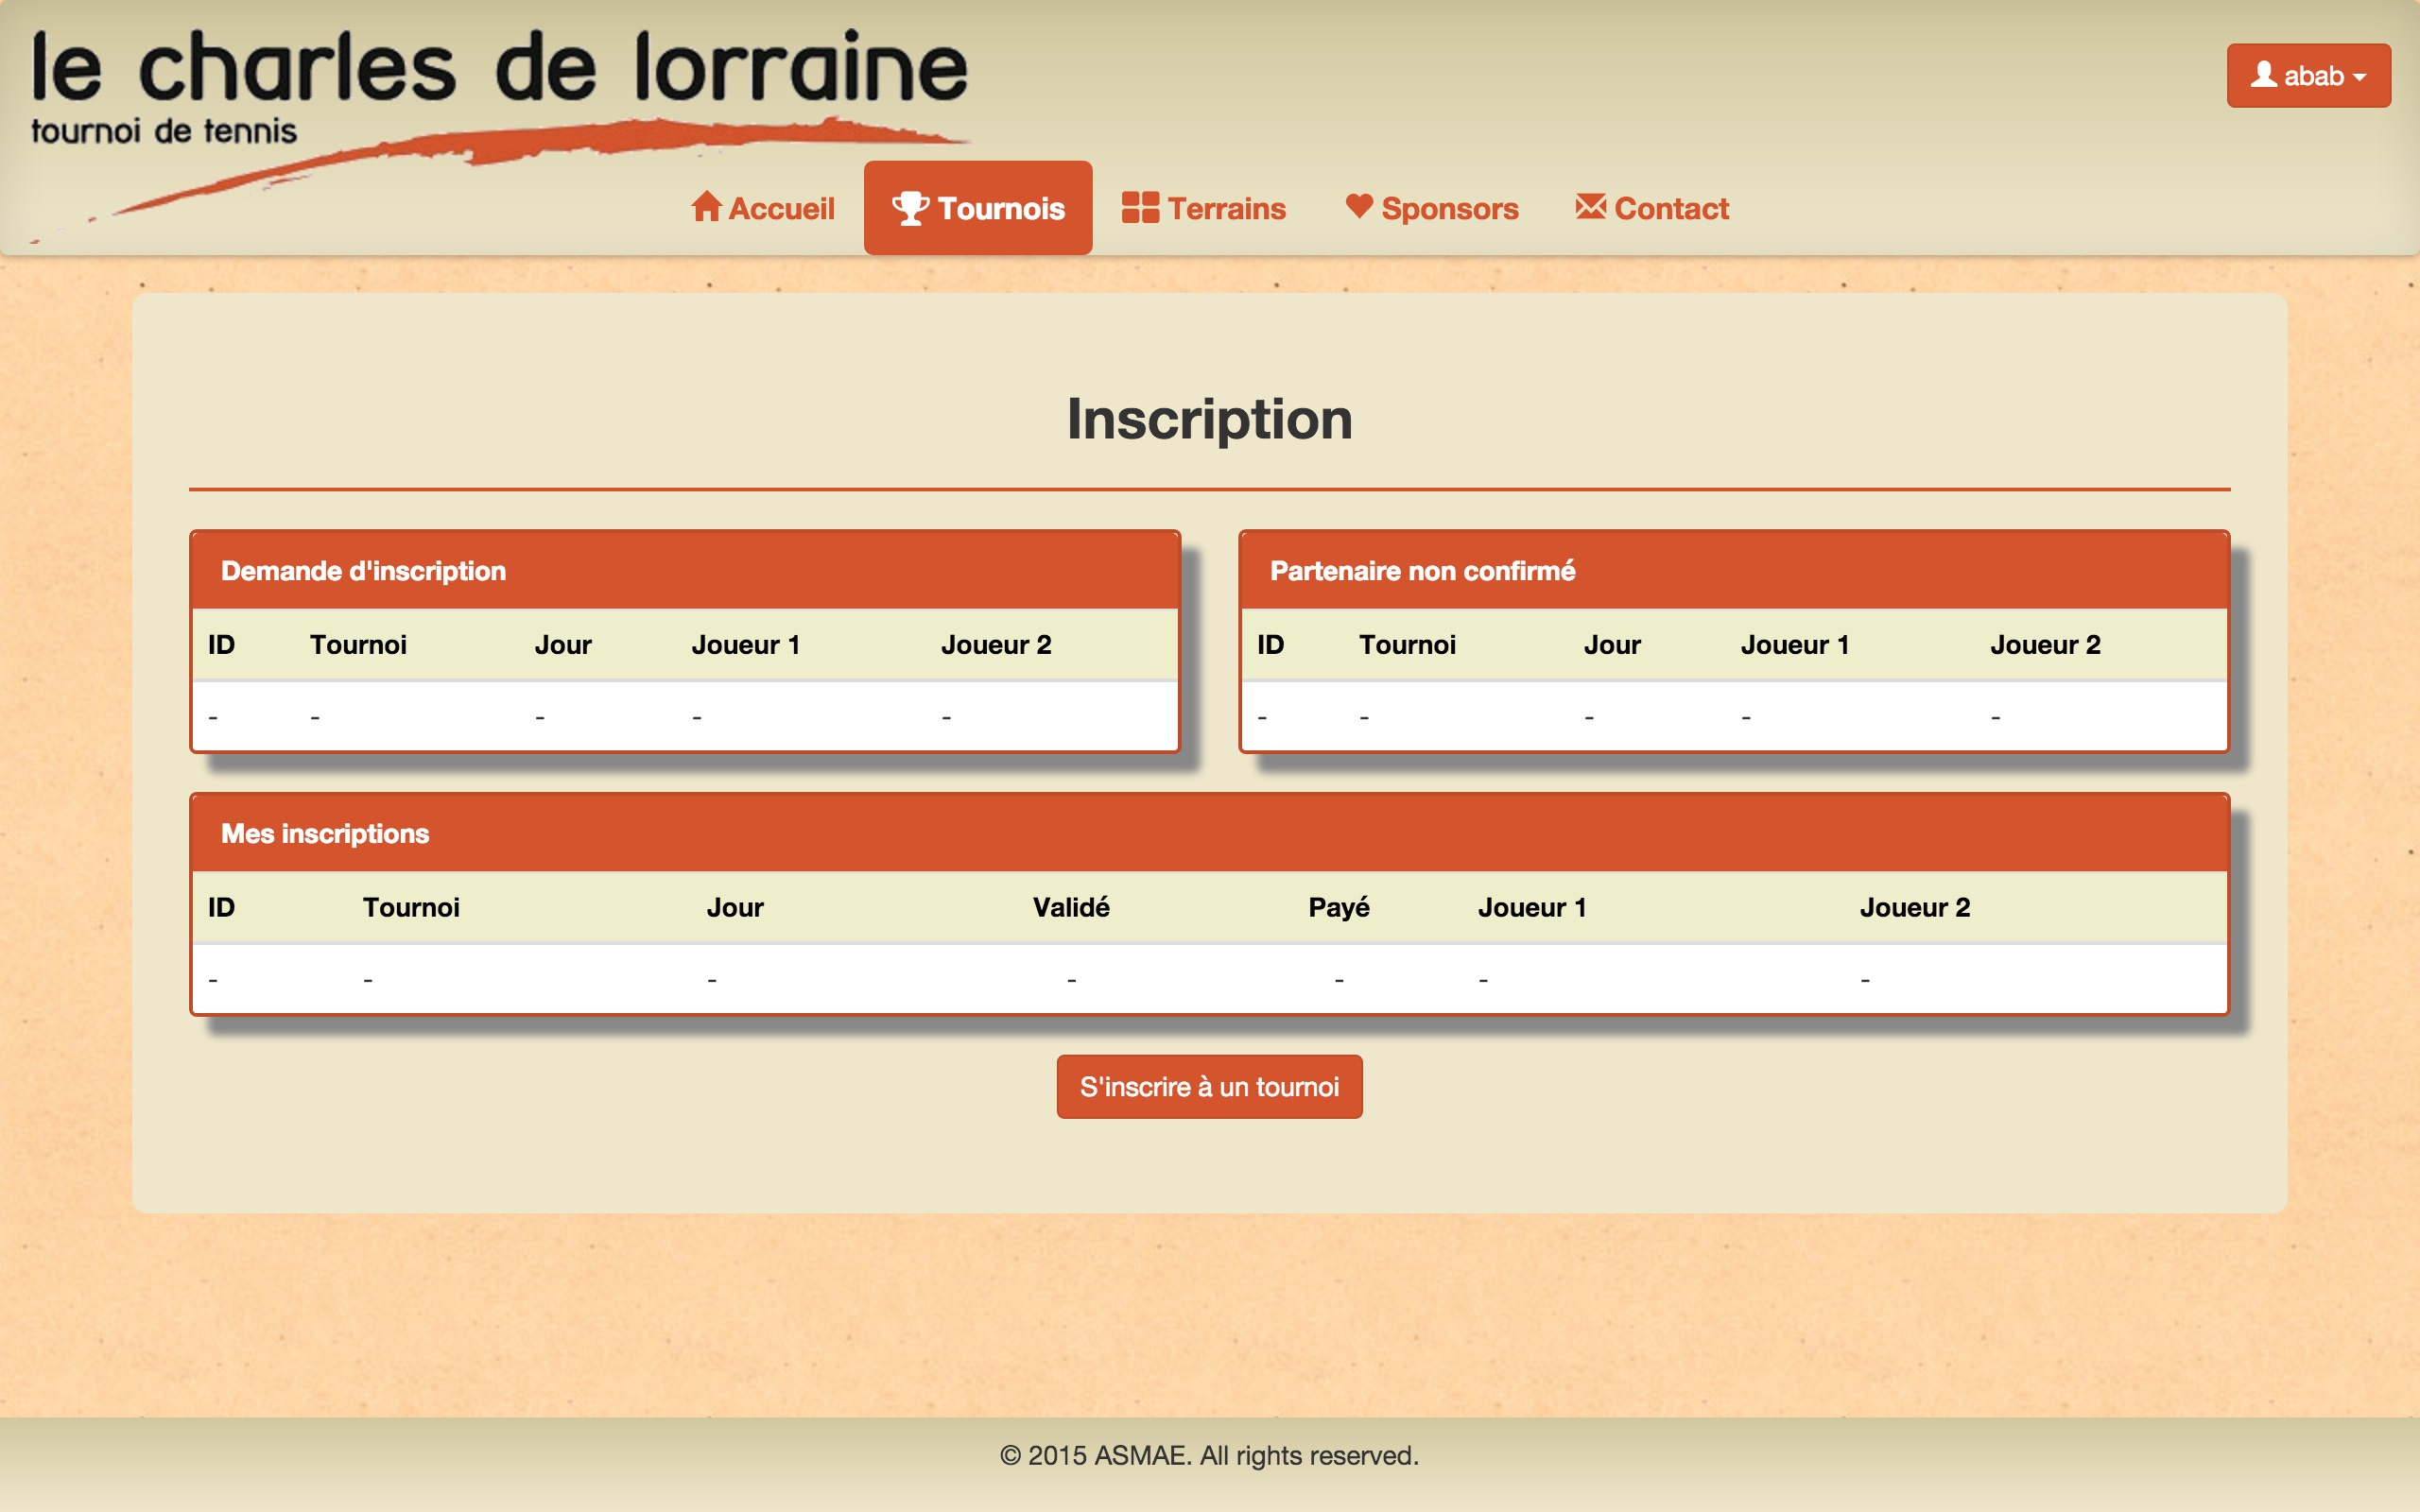
\includegraphics[scale=0.15]{user_images/staff/GererUtilisateurs/ModifierUtilisateur/005.jpg}
\caption{Editer un utilisateur, étape 5}
\end{figure}
